\chapter{Testování}

\section{Uživatelské testy}
Cílem uživatelských testů bylo zjistit, zda mnou zvolené rozhraní bylo správné řešení. Důležitá je totiž intuitivnost rozhraní pro uživatele, aby s ním dokázal pracovat rychle a efektivně.

\subsection{Příprava na test}
Jelikož je certifikace cizích zařízení složitá, zvolil jsem jako testovací přístroj vlastní iPhone, který jsem testovaným osobám dával s připravenou ikonou na obrazovce ke spuštění.

\subsection{Průběh testu}

\subsubsection*{1. kolo}

\begin{enumerate}
	\item Spustit aplikaci
	\item Vstoupit do aplikace jako anonymní uživatel
	\item Změřit jednorázově
	\item Změřit kvalitu sítě
	\item Zobrazit naměřené hodnoty
\end{enumerate}

\subsubsection*{2. kolo}

\begin{enumerate}
	\item Spustit aplikaci
	\item Vstoupit do aplikace jako uživatel se jménem \emph{test} a heslem \emph{test}
	\item Nastavit periodické měření pro každých 30 vteřin
	\item Pustit měření kvality sítě
	\item Minimalizovat aplikaci
	\item Vyčkat 2 minuty
	\item Vrátit se do aplikace a podívat se na doposud naměřené hodnoty
	\item Přerušit měření
\end{enumerate}

\subsection{Vyhodnocení testu}

\begin{table}[h]
	\begin{center}
		\begin{tabular}{|c|c|c|}
			\hline
				{\bf Krok} & {\bf Osoba A} & {\bf Osoba B}\\
			\hline \hline
				1. & OK & OK\\
				\hline
				2. & OK & OK\\
				\hline
				3. & OK & OK\\
				\hline
				4. & OK & OK\\
				\hline
				5. & OK & OK\\
				\hline \hline
				1. & OK & OK\\
				\hline
				2. & OK & OK\\
				\hline
				3. & OK & OK\\
				\hline
				4. & OK & OK\\
				\hline
				5. & OK & OK\\
				\hline
				6. & OK & OK\\
				\hline
				7. & OK & OK\\
				\hline
				8. & OK & OK\\
				\hline
		\end{tabular}
	\end{center}
	\caption{Tabulka úspěšnosti uživatelských testů}
	\label{tab.usr}
\end{table}

Všem dotázaným bylo předem řečeno, že nebude možné odpovídat na jejich dotazy. Osoba B se v případě nastavení periodického měření ptala na překlad, ale nakonec se to obešlo bez komplikací.

\subsubsection{Závěr}
Aplikace byla vyhodnocená jako intuitivní a přehledná. Tyto výstupy hodnotím pozitivně a je to jasný signál, že jde uživatelské rozhraní tou správnou cestou.

\newpage

\section{Funkční testy}

\subsection{Prostředky pro testování}
Součástí SDK pro iOS je simulátor iOS zařízení. Narozdíl od \emph{emulátoru} DVM v SDK \\pro Android, iOS simulátor nepřepočítává procesorové funkce a spouští se velmi rychle. Běh aplikace je simulován věrohodně a rychlost je velmi blízká reálnému zařízení. Pro rozsáhlé testování je ovšem nevhodný, protože neodráží skutečný svět. Neříká nic o výdrži baterie, a zároveň má stálé, pevné připojení k internetu.

Pro účely testování jsem měl mimo simulátor k dispozici zařízení:

\begin{enumerate}
	\item iPhone 5
	\begin{itemize}
		\item O2-CZ
		\item Neomezený datový tarif
		\item iOS 6.1.4 (10B350)
	\end{itemize}
	
	\item iPad 2
	\begin{itemize}
		\item O2-CZ
		\item 10GB FUP
		\item iOS 5.1.1 (9B206)
	\end{itemize}
\end{enumerate}

\begin{figure}[htp]
	\centering
	\label{figur}

  	\subfloat[iPhone 5] {
  		\label{figur:1}
  		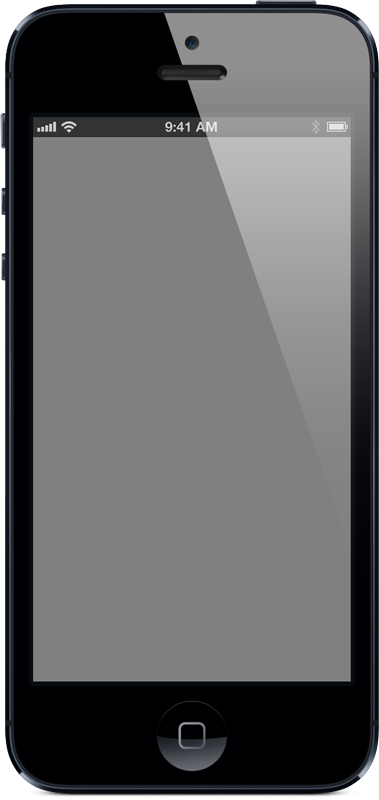
\includegraphics[width=0.18\textwidth]{figures/04_testing/iphone.jpg}
  	}
  		\qquad
  	\subfloat[iPad 2] { 
  		\label{figur:2}
  		
\includegraphics[width=0.3\textwidth]{figures/04_testing/ipad.jpg}
  	}
	\caption{Zařízení k testování} (nejedná se o reálný poměr velikostí)
\end{figure}

\newpage

\subsection{Výdrž baterie}

\subsubsection{Příprava na test}
Pro účely testování výdrže baterie v telefonu jsem využil iPhone 5. Nahrál jsem do něj aktuální verzi aplikace a plně jsem jej nabil. Telefon byl během testu používán v každodenních činnostech - telefonování, psaní sms, elektronická pošta, focení a prohlížení webových stránek.

\subsubsection{Průběh testu}

\subsubsection*{1. kolo}

\begin{enumerate}
	\item Spustit aplikaci
	\item Přihlásit se pod vlastním účtem
	\item Spustit periodické měření na každých 30 vteřin
	\item Minimalizovat aplikaci
	\item Pravidelně kontrolovat, zda aplikace nespadla
	\item Sledovat stav baterie do 5\% nabití
\end{enumerate}

\subsubsection*{2. kolo}

\begin{enumerate}
	\item Spustit aplikaci
	\item Přihlásit se pod vlastním účtem
	\item Spustit periodické měření na každých 15 minut
	\item Minimalizovat aplikaci
	\item Pravidelně kontrolovat, zda aplikace nespadla
	\item Sledovat stav baterie do 5\% nabití
\end{enumerate}

\newpage

\subsubsection{Vyhodnocení testu}
V nepravidelných intervalech jsem kontroloval stav baterie a zaznamenával jej do tabulky v obou kolech. V používání telefonu jsem se nelimitoval.

\subsubsection*{1. kolo}

\begin{table}[h]
	\begin{center}
		\begin{tabular}{|l|c|}
			\hline
				{\bf Čas} & {\bf Stav nabití baterie}\\
			\hline \hline
				13:50 & 98\%\\
				\hline
				14:10 & 97\%\\
				\hline
				14:25 & 95\%\\
				\hline
				14:35 & 93\%\\
				\hline
				14:40 & 91\%\\
				\hline
				14:45 & 90\%\\
				\hline
				15:05 & 85\%\\
				\hline
				15:15 & 82\%\\
				\hline
				15:25 & 78\%\\
				\hline
				15:45 & 72\%\\
				\hline
				15:55 & 70\%\\
				\hline
				16:15 & 65\%\\
				\hline
				16:25 & 62\%\\
				\hline
				16:40 & 59\%\\
				\hline
				16:45 & 58\%\\
				\hline
				17:00 & 55\%\\
				\hline
				17:15 & 51\%\\
				\hline
				17:35 & 46\%\\
				\hline
				17:55 & 42\%\\
				\hline
				18:20 & 35\%\\
				\hline
				18:50 & 28\%\\
				\hline
				19:15 & 23\%\\
				\hline
				19:50 & 16\%\\
				\hline
				19:50 & 9\%\\
				\hline
				20:30 & 5\%\\
				\hline
		\end{tabular}
	\end{center}
	\caption{Tabulka naměřených hodnot stavu nabití baterie - 1. kolo}
	\label{tab.30s}
\end{table}

Telefon se za velice krátkou dobu vybil (necelých 7 hodin). Při intervalu 30 vteřin provedl měření celkem 827krát (nenechal jsem ho měřit do úplného vybití).

\newpage

\begin{figure}[h]
	\centering
	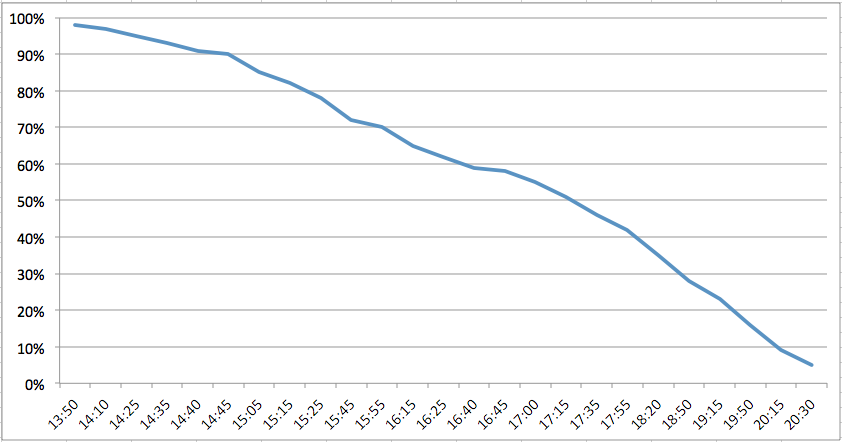
\includegraphics[width=0.8\textwidth]{figures/04_testing/graph30.jpg}
	\caption{Stav baterie vzhledem k času při měření s intervalem 30 vteřin}
	\label{batt1}
\end{figure}

\subsubsection*{2. kolo}
\begin{table}[h]
	\begin{center}
		\begin{tabular}{|l|c|}
			\hline
				{\bf Čas} & {\bf Stav nabití baterie}\\
			\hline \hline
				9:00 & 99\%\\
				\hline
				10:00 & 94\%\\
				\hline
				11:00 & 87\%\\
				\hline
				12:00 & 83\%\\
				\hline
				13:00 & 77\%\\
				\hline
				14:00 & 75\%\\
				\hline
				15:00 & 71\%\\
				\hline
				16:00 & 66\%\\
				\hline
				17:00 & 63\%\\
				\hline
				18:00 & 57\%\\
				\hline
				19:00 & 51\%\\
				\hline
				20:00 & 46\%\\
				\hline
				21:00 & 41\%\\
				\hline
				22:00 & 38\%\\
				\hline
		\end{tabular}
	\end{center}
	\caption{Tabulka naměřených hodnot stavu nabití baterie - 2. kolo}
	\label{tab.15m}
\end{table}

Telefon změřil kvalitu sítě při intervalu 15 minut  92krát. Ve 22:00 měl stále dostatečně nabitou baterii pro standartní používání (38\%).

\newpage

\begin{figure}[h]
  	\centering
    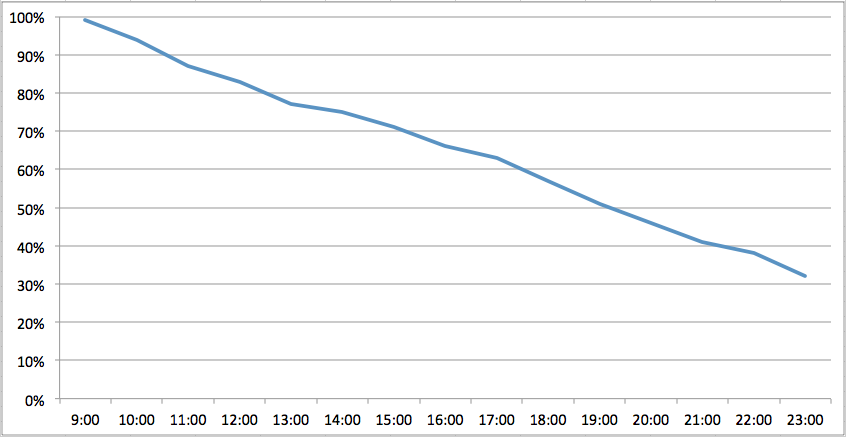
\includegraphics[width=0.8\textwidth]{figures/04_testing/graph15.jpg}
    \caption{Stav baterie vzhledem k času při měření s intervalem 15 minut}
    \label{batt2}
\end{figure}

\subsubsection*{Závěr}
Testy vyhodnocuji pozitivně. Pro měření s velice krátkým intervalem vydrží telefon měřit kvalitu sítě 7 hodin při standartním používání. Pokud bude chtít uživatel měřit s větším intervalem, rozdíl ve výdrži baterie téměř nepozná.

\subsection{Test kvality měření oproti konkurenci}

\subsubsection{Příprava na test}
Pro testování kvality měření oproti konkurenčním aplikacím jsem použil iPhone 5 s nainstalovanými aplikacemi DSL.cz, Speedtest.net a MBTest. Telefon měl v průběhu měření vypnutou WiFi a byl v okruhu dobrého připojení do sítě 3G (FEL ČVUT, Karlovo Náměstí).

\subsubsection{Průběh testu}

\begin{table}[h]
	\begin{center}
		\begin{tabular}{|l|c|}
			\hline
				{\bf Aplikace} & {\bf Naměřená rychlost download/upload}\\
			\hline \hline
				Speedtest.net & 5.61 Mbps/1.16 Mbps\\
				\hline
				DSL.cz & 4.19 Mbps/1.53 Mbps\\
				\hline
				MBTest & 4.70 Mbps/1.26 Mbps\\
				\hline
		\end{tabular}
	\end{center}
	\caption{Tabulka naměřených hodnot měřících aplikací}
	\label{tab.speed}
\end{table}

\subsubsection*{Vyhodnocení testu}
Zpočátku se vyskytly potíže nepřesného měření. Řešením bylo nastavení větší velikosti bufferu na socketu na straně klienta. Výstupy hodnotím kladně a považuji drobné odchylky za zanedbatelné.